%%%%%%%%%%%%%%%%%%%%%%%%%%%%%%%%%%%%%%%%%%%%%%%%%%%%%%%%%%%%%%%%%%%%%%%%%%%%%%%%%%%%%%%%%%%%%%%%%%%%%%%
%%%%%%%%%%%%%% Template de Artigo Adaptado para Trabalho de Diplomação do ICEI %%%%%%%%%%%%%%%%%%%%%%%%
%% codificação UTF-8 - Abntex - Latex -  							     %%
%% Autor:    Fábio Leandro Rodrigues Cordeiro  (fabioleandro@pucminas.br)                            %% 
%% Co-autor: Prof. João Paulo Domingos Silva  e Harison da Silva                                     %%
%% Revisores normas NBR (Padrão PUC Minas): Helenice Rego Cunha e Prof. Theldo Cruz                  %%
%% Versão: 1.0     13 de março 2014                                                                  %%
%%%%%%%%%%%%%%%%%%%%%%%%%%%%%%%%%%%%%%%%%%%%%%%%%%%%%%%%%%%%%%%%%%%%%%%%%%%%%%%%%%%%%%%%%%%%%%%%%%%%%%%
\section{\esp Introdução}

Em um mercado globalizado e competitivo, as tecnologias da informação se tornaram fundamentais para o auxílio da gestão das empresas em suas atividades rotineiras e também no suporte a tomadas de decisões e a possibilidade de desenvolvimento de novos negócios, novos modelos de negócio e a modificação dos valores estratégicos das empresas. \cite{audy}.

Visando a adequação às mudanças mercadológicas, organizacionais e à manutenibilidade em relação a concorrência, o investimento em sistemas de informação tem uma grande parcela do orçamento das empresas, buscando o alinhamento da Tecnologia da informação e negócios. \cite{luftman}  
Para atender a essas necessidades, os requisitos de sistemas têm se tornado cada vez mais complexos, voláteis e robustos diante das demandas das organizações. 
As denominadas metodologias ágeis permitem a entrega de \textit{software} funcionais em ciclos de desenvolvimento mais curtos, considerando a velocidade demandada para a sua construção. \cite{sbbrocco} 
          
No entanto, as equipes que lidam com a infraestrutura têm a difícil tarefa de implantar um \textit{software} em produção a medida em que são criados ou modificados, pois estes sistemas requerem dependências de componentes externos, como configurações de \textit{hardware}, sistemas operacionais, banco de dados, servidores de aplicação e web e ainda configurações específicas da aplicação. Isto demanda um tempo considerável para a implantação destes sistemas.

Para garantir um processo totalmente ágil e que acompanhe as exigências do negócio da organização, é necessário que haja uma integração do desenvolvimento de sistemas e as operações de infraestrutura. Portanto, essa abordagem ágil também deve ser seguida pelas equipes de infraestrutura.
O movimento cultural denominado DevOps surgido em meados de 2009 foi influenciado principalmente por metodologias ágeis e computação na nuvem. Ele teve como fundamento a automatização de processos das operações de infraestrutura e a integração entre as equipes de desenvolvimento e operações. \cite{sato}.

A automatização de processos de infraestrutura é uma das premissas do DevOps, utilizando uma abordagem para provisionar e gerenciar recursos de computação como máquinas virtuais, discos de armazenamento, regras de segurança, instalação de \textit{software}, regras de redes e qualquer outro componente de serviço, destinando-se a simplificar significativamente a configuração e o gerenciamento de recursos. Ao tratar a infraestrutura como código, as organizações podem usar as melhores práticas de desenvolvimento de software, incluindo revisão de código e controle de versão, documentação e testes. Esta abordagem reduz a complexidade do gerenciamento, pois todo o processo é dividido em tarefas em menores e mais processos gerenciáveis.A abordagem da infraestrutura como código ou também conhecida como IaC reduz os riscos operacionais, permitindo revisar o código e salvar todas as revisões anteriores de uma infraestrutura codificada, podendo restaurar a infraestrutura em qualquer revisão anterior, quando necessário.

Segundo \citeonline{Morris:2016:ICM:3006361}, a essência da infraestrutura como código é submeter a configuração da infraestrutura da mesma maneira que o código fonte do software é tratado, usando sistemas de gerenciamento de código-fonte, \textit{TDD} \footnote{\textit{TDD - Test Driven Development}: O teste são que são escritos antes do nosso código de produção} , integração contínua \footnote{\textit{CI - Continuous Integration}: É uma prática de desenvolvimento de \textit{software} em que os desenvolvedores, juntam suas alterações de código em um repositório central e os testes são executados. Geralmente, a integração contínua se refere ao estágio de criação ou integração do processo de lançamento de software  }, refatoração de código e outras técnicas, que são úteis para garantir que as alterações na infraestrutura sejam exaustivamente testadas, repetíveis e transparentes.

\subsection{Problema}

O problema a ser resolvido é baseado em cenário onde a automação de infraestrutura é atualmente ineficiente, em que a equipe não conseguem acompanhar a carga de mudanças, acarretando em um tempo considerável da equipe para disponibilizar recursos e para dificultar ainda não tem conhecimento ou experiência sobre infraestrutura como código e suas ferramentas e ainda um outro agravante e que existem inúmeras ferramentas disponíveis no mercado, o que acaba intensificando a dificuldade de adoção de alguma ferramenta. Conforme indicado neste artigo, ele traz um comparativo entre ferramentas para que auxiliem a equipe a ter um certo conhecimento e confiança para adoção de alguma apresentada. Vale ressaltar que só adoção de uma ferramenta não resolverá o problema como todo e deve ser integrada com outras ferramentas quando necessário.  


  Como motivação os benefícios com a implantação de ferramentas permite-se:  
\begin{itemize}
 \item Eficiência no controle dos recursos, sabendo por exemplo, quais recursos uma aplicação usa;
 \item Adaptabilidade da infraestrutura aos requisitos da aplicação;
 \item Os próprios desenvolvedores podem definir , provisionar e gerenciar os recursos de que precisam, sem precisar da equipe de infraestrutura para fazer isso por eles;

\item As equipes serão capazes de se recuperar fácil e rapidamente das falhas, em vez de assumir que a falha pode ser completamente evitada;

\item Permite que ambientes inteiros sejam replicados;

\item Permitir que se teste a infraestrutura antes de ser disponibilizada em um cenário real;
\end{itemize} 


\subsection{Objetivos}

Neste artigo será apresentado uma abordagem geral de \textit{IAC}, um comparativo entre duas ferramentas e apresentar os resultados obtidos e uma conclusão. Os objetivos específicos serão explicar as diferenças entre \textit{softwares} de gerenciamento de configuração e \textit{softwares} de provisionamento, infraestrutura imutável e mutável, descrever e avaliar as características de cada ferramenta escolhida e apresentar resultados. Este trabalho não abordará itens como: integração de ferramentas \textit{IAC} com ferramentas de \textit{CI}, aplicações de metodologias de desenvolvimento de software. 

\subsection{Contextualização}
Os processos de desenvolvimento passaram por uma transformação ao longo dos anos, devido aos movimentos ágeis que mudaram a maneira como as equipes interagem na construção de sistemas, focando cada vez mais em qualidade e entrega de produtos incrementais. Para responder rápido a essas mudanças, um processo de desenvolvimento deve ser bem definido e bem estabelecido, o que compreende desde a etapa de desenvolvimento, teste e a entrega. No entanto, estabelecer estas etapas podem ser difíceis, uma vez que os recursos(financeiro, pessoal e tempo) competem com as demandas de entregas do sistema. A medida em que os sistemas são evoluídos a complexidade dos requisitos aumenta e do ponto de vista da parte da infraestrutura, um sistema pode necessitar, por exemplo, que ele seja distribuído, exigir centenas de máquinas para o funcionamento e uma grande capacidade de processamento. E se o ciclo de provisionamento e gerenciamento de infraestrutura não estiver totalmente automatizado, um grande tempo será gasto para gerenciar recursos, que são geralmente distribuídos em tarefas rotineiras e repetitivas o que pode se tornar um empecilho para que as entregas cheguem até o cliente. 

Desenvolver uma infraestrutura que seja totalmente resiliente e automatizada, seguindo os princípios de práticas \textit{DevOps}, não é uma tarefa fácil considerando um ambiente computacional na nuvem, onde os recursos são ilimitados e escaláveis e que exigem uma mudança de paradigma e novas habilidades para se trabalhar com \textit{cloud}.  


\section{\esp Metodologia}

A escolha das ferramentas obedeceram critérios da tabela de \citeonline{masek} e dentre as ferramentas que atendem às características descritas na tabela, foram escolhidas o \textit{Ansible} e o \textit{Terraform} usando critérios extras como aceitação do mercado, suporte comercial e maturidade da ferramenta.

Para medir a aceitação do mercado foram realizadas pesquisas em sites especializados de comparação de tipos de ferramentas. Um outro aspecto consideração foi se é uma ferramenta \textit{open source}(um ponto importante para permitir adaptação da ferramenta),se possui um plano de suporte pago, para critério de desempate foi considerado o preço do suporte. Para medir a maturidade foram considerados o tempo de mercado, documentação, tempo de lançamento entre versões e a integração com outras ferramentas.

A realização dos testes foram consideradas as últimas versões estáveis de lançadas no momento da escritas desse artigo, o \textit{Ansible}(2.4.6) e o \textit{Terraform}(0.12.13). Os testes foram usando o fornecedor de computação na nuvem  \textit{Digital Ocean}. \footnote{https://www.digitalocean.com/}   

As métricas comparativas consideradas foram a linguagem de escrita, a performance(o tempo em que cada ferramenta leva para criar um determinado número de recursos. O controle de estado(capacidade da ferramenta  de controlar e identificar o estado real dos recursos) e a extensibilidade da ferramenta(Se possui um conjunto de \textit{SDK's} \footnote{\textit{SDK - Software Development Kit}} em que permite a programadores estender as funcionalidades da ferramenta).  


\section{\esp Trabalhos Relacionados} \label{relacionados}


\citeonline{Carnegie} explicam que o \textit{design} da infraestrutura é a fase do ciclo de vida do produto em que se define e configura os recursos necessários para o funcionamento dele. A Infraestrutura como código é um conjunto de práticas que usam código para configurar recursos, como máquinas e redes (virtuais), instalar programas, configurar um banco de dados e definir uma regra de segurança. As práticas IaC permitem a criação de vários recursos de maneira automatizada e padronizada, controlando o estado da infraestrutura, além disso permitem o controle de versão, ou seja, pode-se desfazer de qualquer mudança na infraestrutura, somente alterando o código do recursos. Ele também cita que antes mesmo do surgimento da IaC os administradores de sistemas já utilizavam automação, através de \textit{script} para realizar as tarefas de configuração de infraestrutura. E que a IaC surgiu com a popularização da computação da nuvem como serviço e que todos os recursos oferecidos são virtuais. No artigo ele ainda descreve que os provedores de serviços em nuvem fornecem um console de gerenciamento(uma interface \textit{web}) para a administração de recursos. Porém, para um sistema de larga escala, usar o console não é muito prático, devido à dificuldade de gerenciar centenas de recursos que são criados e destruídos com uma grande frequência. Deve-se usar as \textit{application program interface} \footnote{É um conjunto de rotinas e padrões de programação para acesso a um aplicativo de \textit{software} ou plataforma baseada na \textit{Web}, permitindo que dois aplicativos se comuniquem. } (API) disponibilizadas pelo provedor ou ferramentas IaC que interagem com essas API que resolvem a questão da criação e destruição de alta frequência desses recursos. Por fim, ele cita a relação entre infraestrutura como código \textit{Agile} e o DevOps. 

\hfill

Segundo \citeonline{masek}, a popularização da virtualização e o crescente poder dos servidores e a disponibilidade da computação em nuvem levaram a um aumento significativo no número de servidores e estações de trabalho que precisam ser gerenciados. Nesse ponto, as ferramentas de gerenciamento de orquestração e gerenciamento de configuração se aplicam nesses casos. Os administradores de sistema gerenciam grupos de servidores ou estações de trabalho idênticas (máquinas físicas ou máquinas virtuais) que executam aplicativos e serviços idênticos. Em seu artigo ele apresenta um estudo sobre o uso da ferramenta \textit{Ansible} nos laboratórios da \textit{Brno University of Technology (BUT)}. Ele descreve que o objetivo de utilizar uma ferramenta de IaC é fornecer uma plataforma para gerenciar com eficiência a infraestrutura de larga escala dos laboratórios universitários, com o mínimo de contribuição de desenvolvedores ou administradores.
O autor cita dois grupos de ferramentas de infraestrutura como código mais populares: \textit{Chef, Puppet, Ansible e SaltStack}, sendo todas “ferramentas de gerenciamento de configuração”, o que significa que elas foram projetadas para instalar e gerenciar \textit{software} em servidores e estações de trabalho já existentes. E as ferramentas \textit{CloudFormation, Terraform} são “ferramentas de orquestração”, o que significa que eles são projetados para provisionar os servidores.

\hfill

 \citeonline{steve} menciona da importância de escolher ferramentas de IaC, como por exemplo, \textit{ Chef, Ansible, Puppet, SaltStack, Terraform } se deve levar em consideração o conjunto de casos em que essas ferramentas se propõem a resolver. Estas ferramentas são classificadas em dois domínios: gerenciamento de configurações e orquestração de configuração e quais casos elas resolvem. O autor ainda explica os conceitos de infraestrutura mutável e imutável, escrita de código procedural e declarativa. Este conceitos serão abordados na seção \ref{IaC}. 

\citeonline{steve} expressa que se deve escolher uma ferramenta focada na orquestração de infraestrutura e outra em gerenciamento de configuração de aplicativos reunindo os benefícios de ambas, pois os desafios do gerenciamento de provisionamento e configuração estão intimamente relacionados, porque as organizações geralmente provisionam os servidores e implantam aplicativos neles. Sendo que neste ponto os tipos de ferramentas de IaC vão se convergir.   

\section{\esp IaC ou Infraestrutura como código} \label{IaC}

Os items apresentados neste capítulo foram levantados de acordo com assuntos abordados na seção \ref{relacionados}. A ideia dessa seção é descrever os conceitos básicos da infraestrutura como código de forma sucinta para um entendimento geral do assunto.  

\subsection{Tipos de Ferramentas IaC}
As ferramentas de gerenciamento de configuração como \textit{Chef, Puppet, Ansible,Saltack} foram projetadas para instalar e gerenciar softwares em servidores já existentes. Por exemplo, na instalação de um banco de dados, adicionar uma regra de \textit{firewall}, realizar uma atualização no sistema operacional. 

As ferramentas de Provisionamento como \textit{Terraform, Heat, Cloudformation} e foram projetadas criar as próprias instâncias \footnote{Uma instância é um servidor virtual na nuvem. Por exemplo: Uma instância rodando o sistema operacional LINUX} e a inicialização de seus recursos. 

Segundo \citeonline{Carnegie}, existem sobreposições e esses termos não são mutuamente exclusivos para ambas as ferramentas. As ferramentas de provisionamento podem realizar tarefas de configuração e ferramentas de configuração podem realizar tarefas de provisionamento, porém elas se concentram naquilo que são melhores. 

Ambas as categorias de ferramentas utilizam dois modelos para descrever os recursos, um tipo se concentram no resultado final , já o outro tipo é preciso descrever os passos necessários para atingir o resultado final. O resultado final pode ser entendido como por exemplo, criar uma nova máquina ou instalar uma versão do java. 

\subsection{Linguagem}

As ferramentas de IaC usam arquivos de definição como \textit{DSL} \footnote{\textit{DSL - Domain-Specific Language:} Uma linguagem de domínio específico é criada especificamente para resolver problemas em um domínio particular e não se destina a ser capaz de resolver os problemas fora de seu âmbito. }, ou formatos de texto conhecidos comuns como, \textit{ YAML} \footnote{\textit{YAML - Ain't  Markup Language}: É um formato de serialização (codificação de dados) de dados legíveis por humanos -  https://yaml.org/ }, \textit{JSON} \footnote{\textit{JSON - JavaScript Object Notation:} É uma formatação leve de troca de dados. Para seres humanos, é fácil de ler e escrever. Para máquinas, é fácil de interpretar e gerar. Está baseado em um subconjunto da linguagem de programação JavaScript, https://www.json.org/json-pt.html}, \textit{XML} \footnote{\textit{XML - eXtensible Markup Language:} é uma linguagem de marcação para a criação de documentos com dados organizados hierarquicamente, tais como textos, banco de dados ou desenhos vetoriais.}
  ou linguagens de programação como, \textit{Python} \footnote{\textit{Python} é uma linguagem de programação de alto nível, interpretada, de script, imperativa, orientada a objetos, funcional, de tipagem dinâmica e forte.}  \textit{Ruby} \footnote{\textit{Ruby} é uma linguagem de programação interpretada multi-paradigma, de tipagem dinâmica e forte, com gerenciamento de memória automático.}  ou uma mesclagem de ambas.
  
  Elas se concentram em dois tipos de estilo de escrita de código: 
   \begin{itemize}
       \item Declarativo: É o modelo em que é um recursos é especificado e o estado final desejado a própria ferramenta de Iac é responsável por descobrir como atingir estado estado. Veja o exemplo na Figura \ref{fig:figura2}.
   \end{itemize}

 \begin{itemize}
    \item Procedural: É o estilo na qual você escreve um código e especifica, passo a passo, como atingir o estado final desejado. O usuário deve deve determinar o processo de implantação ideal. Veja o exemplo na Figura \ref{fig:figura1}.
   \end{itemize}
   
 \begin{figure}[ht]
	\centering	
	\caption[\hspace{0.1cm}Exemplo declarativo]{Exemplo de escrita declarativa da ferramenta Terraform}
	\vspace{-0.4cm}
	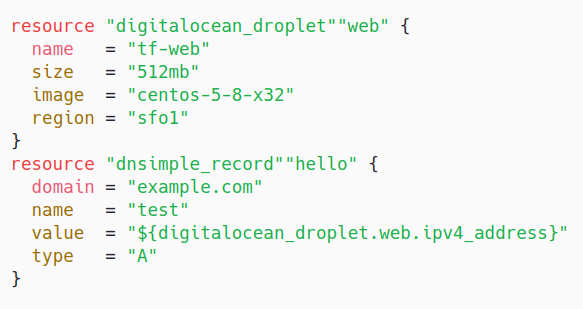
\includegraphics[width=0.98\textwidth]{artigo/figuras/terraform-declarative-exemple-01.png}
	 \vspace{-0.2cm}
	\\\textbf{\footnotesize Fonte: \cite{terraform01} }
	\label{fig:figura2}
\end{figure}
\vspace{-0.5cm}
 
\begin{figure}[h]
	\centering	
	\caption[\hspace{0.1cm}Exemplo procedural]{Exemplo de escrita procedural da ferramenta Chef}
	\vspace{-0.4cm}
	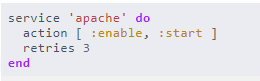
\includegraphics[width=0.5\textwidth]{figuras/chef-io-exemplo-procedural.png}
	 \vspace{-0.2cm}
	\\\textbf{\footnotesize Fonte: \cite{chef01}}
	\label{fig:figura1}
\end{figure}
\vspace{-0.5cm}

 \subsection{Tipos de Infraestrutura}
 
 Nesta seção são abordadas duas característica de como as infraestruturas são tratadas atualmente e apresentar uma a ideia central dos conceitos. Não serão discutidos qual modelo é melhor ou qual as vantagens de se utilizar um ou outro. 

 Segundo \citeonline{Morris:2016:ICM:3006361}, na infraestrutura mutável, a cada mudança de algum componente, seja por uma demanda de serviço, aplicação, segurança, estas atualizações precisam ser replicadas em todos os servidores que dependem dessas mudanças. A medida que atualizações são realizadas, cada servidor tem um histórico único de alterações, possuindo sutis diferenças de configuração. As ferramentas de gerenciamento de configuração normalmente são padronizadas para este paradigma de infraestrutura mutável. 
 
  Um exemplo hipotético seria a migração do \textit{JAVA}\footnote{Java é uma linguagem de programação e plataforma computacional.} para uma versão superior. Na infraestrutura mutável cada servidor precisaria receber esta atualização do JAVA. A infraestrutura mutável é como a maioria dos ambientes computacionais funcionam hoje.
 
 Segundo \citeonline{Dadgar}, a noção de imutabilidade é a ideia de que, uma vez criada uma coisa, não a mudamos após a criação.
 Na infraestrutura imutável qualquer alteração a ser realizada deve ser feita através da substituição completa dos servidores. Estas alterações são feitas criando novas configurações e novos servidores são criados a partir delas. Isso aumenta a previsibilidade porque este servidor já foi testado antes de ir para a produção. Em outras palavras, as implantações se tornam atômicas. As ferramentas de provisionamento desempenham este papel.\cite{Morris:2016:ICM:3006361}.
 
 Seguindo o mesmo exemplo de atualizar o JAVA. Em modelo de infraestrutura imutável, um novo servidor seria criado com essa atualização e testado e então, os antigos seriam destruídos e substituídos por novos. A infraestrutura imutável só faz sentindo em um ambiente virtualizado. 
 
\subsection{Arquitetura}

Nesta seção é apresenta dois conceitos de como as ferramentas foram projetadas para funcionar. Não serão discutidos ou comparados qual o melhor modelo ou suas vantagens e desvantagens. 

\subsubsection{Cliente ou Masterless} \label{semagent}
Segundo \citeonline{Jan-Piet}, conforme citado por \citeonline{Morris:2016:ICM:3006361}, na arquitetura cliente não existe um servidor central e não é necessário instalar agentes nos nós gerenciados, o que torna a configuração mais simples. A configuração é feita escolhendo uma máquina e instalando o cliente e informando os IP's \footnote{\textit{Internet Protocol}} dos nós. A autenticação é feita por meio do protocolo \textit{SSH} \footnote{\textit{SSH - Sever Secure Shell:}  É um protocolo de rede criptográfico para operação de serviços de rede de forma segura sobre uma rede insegura, permitindo a execução remota de comandos.}. Ao alterar algum recurso, ele se conecta ao no \textit{IP} e executa as alterações. Veja a Figura  \ref{fig:figura3}. 

\begin{figure}[ht]
	\centering	
	\caption[\hspace{0.1cm}Exemplo arquitetura Cliente]{Exemplo geral de arquitetura Cliente}
	\vspace{-0.4cm}
	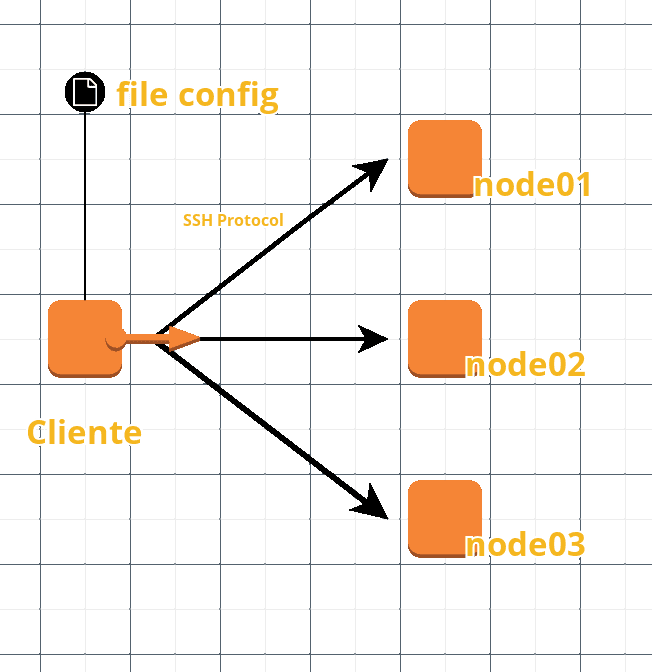
\includegraphics[width=0.5\textwidth]{figuras/cliente.png}
	 \vspace{-0.2cm}
	\\\textbf{\footnotesize Fonte: Próprio Autor}
	\label{fig:figura3}
\end{figure}
\vspace{-0.5cm}


As ferramentas de provisionamento se comunicam diretamente com a \textit{API} do provedor de serviços de nuvem \footnote{Um provedor de serviços de nuvem é uma empresa contratada que fornece uma plataforma, infraestrutura, aplicativo ou serviços de armazenamento baseados em nuvem. Por exemplo: \textit{Amazon Web Service, Azure, Digital Ocean, Google Cloud.}. Eles também são conhecido pelo termo \textit{IaaS - Infrastructure as a service} }


\subsubsection{Mestre/Agente ou Cliente/Servidor} \label{cliente-servidor}
 
 Segundo a \citeonline{puppetlabs}, nessa arquitetura (Figura \ref{fig:figura4}), um servidor \footnote{Dependendo da ferramenta o \textit{master} pode ser representado por mais de um servidor} central denominado mestre controla as informações de configuração de cada nó(cada servidor tem instalado  um agente, geralmente rodando como um processo em segundo plano \footnote{Processos em que não há interação com o usuário}). Este agente solicita seu próprio catálogo de configuração ao mestre.  
 
 Periodicamente, cada agente envia informações ao mestre e solicita um catálogo. O mestre compila e retorna o catálogo de alterações desse nó, usando várias fontes de informações às quais ele tem acesso. Ao receber este catálogo com as alterações a serem realizadas, o agente aplica as alterações no nó. 
 
 Em outras palavras, o fluxo básico de funcionamento é: quando se altera as definições de um recurso, por exemplo, uma nova versão do \textit{Apache} \footnote{É um servidor \textit{web}, compatível com o protocolo HTTP, mantido pela \textit{Apache Software Foundation }}, estas são submetidas para o mestre. Quando o Agente solicita informações do mestre, o mestre compila e retorna um catálogo com as alterações para o nó desse agente usando as fontes de informação às quais o mestre tem acesso. O agente recebe essas alterações e as aplica no nó correspondente, alterando a versão do \textit{Apache}.   

Essa arquitetura pode ter uma leve variação entre ferramentas, podendo ter uma máquina exclusiva de onde o mestre é acessado.

Embora essas ferramentes podem ser usada para o gerenciamento de estações de trabalho não é o objetivo deste estudo. 
\textit{Puppet} e \textit{Chef} são exemplos de ferramentas que são baseadas nesse modelo de arquitetura. 


 \begin{figure}[ht]
	\centering	
	\caption[\hspace{0.1cm}Exemplo arquitetura Master/Agent]{Exemplo geral de arquitetura Master/Agent}
	\vspace{-0.4cm}
	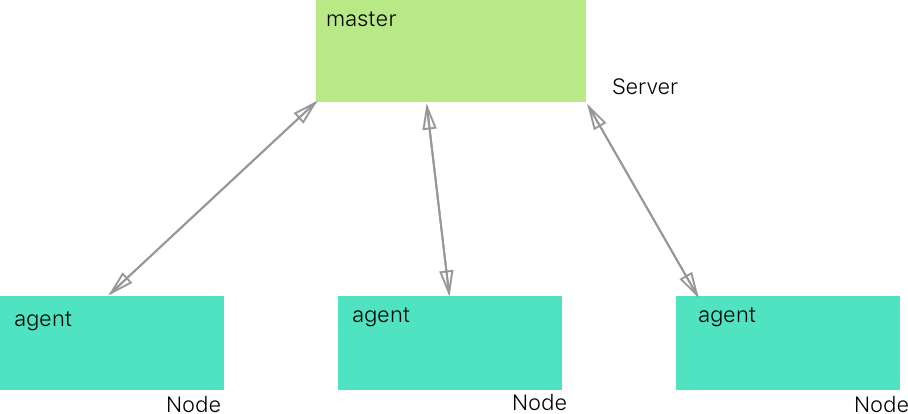
\includegraphics[width=0.5\textwidth]{figuras/master-agent.png}
	 \vspace{-0.2cm}
	\\\textbf{\footnotesize Fonte: \cite{Harit}}
	\label{fig:figura4}
\end{figure}
\vspace{-0.5cm}

\section{Ferramentas}

Esta seção aborda os principais conceitos das ferramentas utilizadas neste artigo. \textit{Ansible} e \textit{Terraform} operam usando uma arquitetura sem agente(conforme mencionado no item \ref{semagent}) e promovem uma interface simplificada legível para a definição de recursos, facilitando a adoção. As definições de conceitos foram retirados diretamente da documentação oficial das ferramentas.

\subsection{Ansible}

A \citeonline{redhat}, descreve o \textit{Ansible} como uma suíte completa de automação de processos de TI simples. Ele abrange desde o provisionamento e o gerenciamento de configurações e outras necessidades.

Ele não usa agentes e nenhuma infraestrutura de segurança personalizada adicional(uma característica de ferramentas, conforme mencionado no item \ref{cliente-servidor}), por isso é relativamente fácil de implantar. O \textit{Ansible} usa uma linguagem de marcação muito simples, o \textit{YAML}, o que é chamado como \textit{Ansible Playbooks} e o estilo de escrita de código é a procedural(\ref{procedural}). E é através dos \textit{Playbooks} que define -se os recursos, estas definições se aproximam de uma escrita em inglês. 

O \textit{Ansible} é descentralizado e depende das credenciais existentes do sistema operacional para controlar o acesso à máquinas remotas. A principal e mais usada forma dele se conectar é usando o protocolo \textit{SSH}.Se necessário, ele pode se conectar facilmente por \textit{Kerberos} \footnote{É um protocolo desenvolvido para fornecer poderosa autenticação em aplicações usuário/servidor, onde ele funciona como a terceira parte neste processo, oferendo autenticação ao usuário.}, \textit{LDAP} \footnote{\textit{LDAP - Lightweight Directory Access:} É um protocolo de aplicação aberto para acessar e manter serviços de informação de diretório distribuído sobre uma rede de IP, permitindo o compartilhamento de informações sobre usuários, sistemas, redes, serviços e aplicações através da rede.} e outros sistemas de gerenciamento de autenticação centralizados.


\textit{Ansible} nasceu como uma ferramenta de gerenciamento de configurações e a partir da versão 2.0 passou a ser uma suíte completa, também podendo provisionar infraestrutura.

 O \textit{Ansible} apresenta os seguintes itens em sua arquitetura:

\hfill
 \begin{itemize}
\item \textbf{\textit{Controller Machine}}: É a máquina de onde o \textit{Ansible} está sendo executado. 

\item \textbf{\textit{Modules}}: Um módulo normalmente abstrai uma tarefa do sistema, por exemplo, instalar um determinado aplicativo e o configurar. Um módulo pode ser escrito em qualquer linguagem de programação. Para usar um módulo, basta referenciar este módulo em alguma tarefa. Os módulos são executados diretamente em um nó.   

\item \textbf{\textit{Plugins}}: Os \textit{plugins} permitem extender as funcionalidades e recursos do \textit{Ansible}, por exemplo, um \textit{plugin} para o envio de \textit{e-mail}. Os \textit{plugins} devem ser escritos em \textit{Python}. Diferente dos módulos, os \textit{plugins} são executados na máquina de controle.

\item \textbf{\textit{Inventory}}: É um arquivo de configuração que contém informações sobre os nós(servidores) que o \textit{Ansible} esta gerenciando. Todos os servidores gerenciados devem ser informados nesse arquivo.

\item \textbf{\textit{Playbooks}}: É o principal ponto de entrada para definir os recursos, escritos por meio do formato \textit{YAML}.

\item \textbf{\textit{Role}}: Uma maneira predefinida de organizar \textit{playbooks} e outros arquivos para facilitar o compartilhamento e a reutilização.

\item \textbf{\textit{Play}}: Uma execução de um \textit{playbook} do início ao fim.

\item \textbf{\textit{Facts}}: Variáveis globais que contêm informações sobre o sistema, como interfaces de rede ou sistema operacional.

\item \textbf{\textit{Task}}: Um bloco de código que define um único procedimento a ser executado, por exemplo, instalar o \textit{Apache}.
 \end{itemize}
 \begin{figure}[ht]
	\centering	
	\caption[\hspace{0.1cm}Exemplo de funcionameno do Ansible]{Exemplo de funcionameno do Ansible}
	\vspace{-0.4cm}
	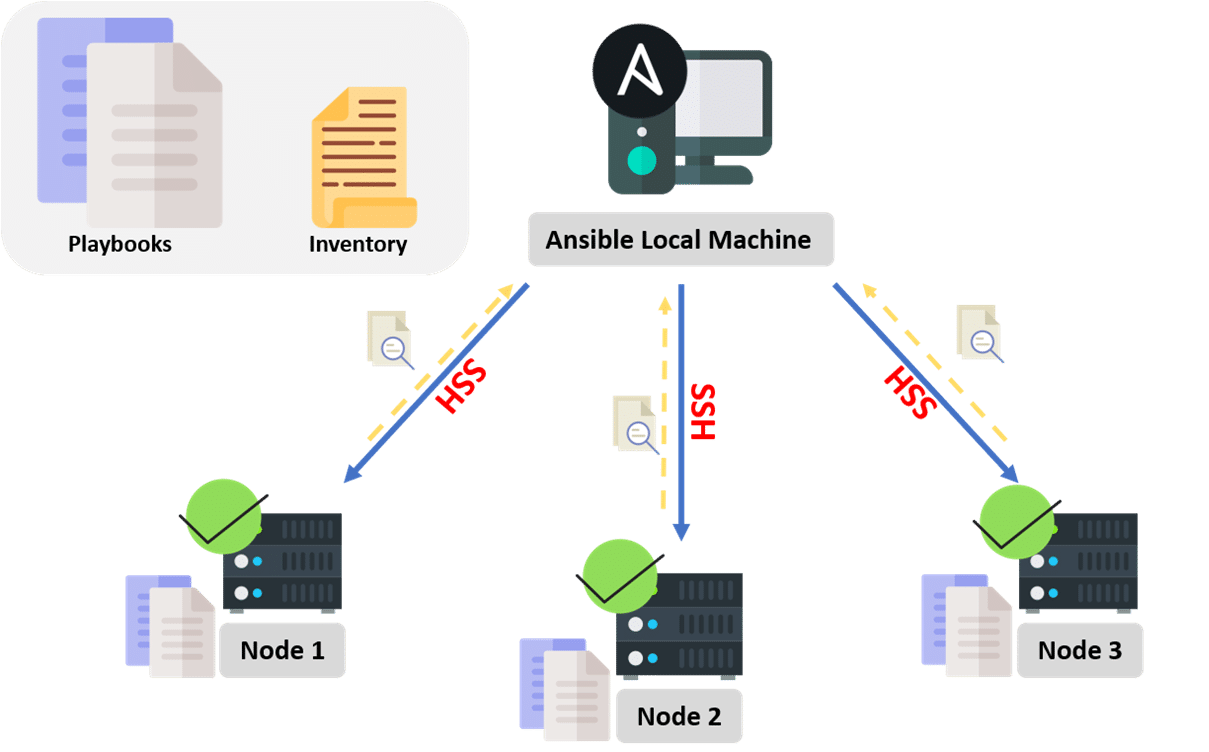
\includegraphics[width=0.5\textwidth]{figuras/ansible-working.png}
	 \vspace{-0.2cm}
	\\\textbf{\footnotesize Fonte: \cite{intellipaat}}
	\label{fig:figura6}
\end{figure}
\vspace{-0.5cm}

\subsection{Terraform} \label{terraform} 

 Segundo a \citeonline{hashcorp2}, o \textit{Terraform} é uma ferramenta para provisionamento de infraestrutura, que permite criar, alterar e criar versões de infraestrutura com segurança e eficiência. Ele pode gerenciar os mais populares provedores de nuvem e também trabalhar com soluções internas personalizadas.

O \textit{Terraform} usa uma linguagem \textit{DSL} muito simples, a \textit{HCL} \footnote{\textit{HCL - Hashicorp Configuration Language.} Veja mais em: \href{https://www.terraform.io/docs/configuration/syntax.html}{https://www.terraform.io/docs/configuration/syntax.html} } (veja na Figura \ref{fig:figura2}) com a extensão de arquivo \textit{"*.tf"} para a definição de recursos de infraestrutura. 

Os arquivos de configuração descrevem para o \textit{Terraform} os componentes necessários para criar um único aplicativo ou toda a configuração da infraestrutura. Ao executar, ele gera um plano de execução descrevendo o que fará para atingir o estado desejado e, em seguida, executa-o para construir a infraestrutura descrita. 
À medida que a configuração muda, ele determina o que mudou e cria planos de execução incrementais para serem aplicados.

Uma característica do \textit{Terraform} é garantir que ao executar um arquivo de definição de recursos varias vezes, o resultado será o mesmo, ou seja, a \textbf{idempotência} \footnote{É a propriedade que algumas operações têm de poderem ser aplicadas várias vezes sem que o valor do resultado se altere após a aplicação inicial.} de uma operação.

O \textit{Terraform} pode criar e gerenciar componentes de baixo nível, como instâncias de servidores, armazenamento e componentes de alto nível(aqui o \textit{Terraform} se sobrepõe com ferramentas de gerenciamento de configuração), como configurar um \textit{DNS} \footnote{\textit{DNS -Domain Name System}: É responsável por localizar e traduzir para números IP os endereços dos sites que digitamos nos navegadores.} de uma máquina.

Além disso o \textit{Terraform} pode ser integrado com as ferramentas de gerenciamento de configuração, como \textit{Ansible, Chef ou Puppet}

Os principais conceitos dele são:
 \begin{itemize}
\item \textbf{Infraestrutura como código}: A infraestrutura é descrita usando uma sintaxe de configuração de alto nível. Isso permite que os recursos da infraestrutura sejam versionados e tratados como qualquer outro código. Além disso, a infraestrutura pode ser compartilhada e reutilizada.

\item \textbf{Planos de Execução}: O \textit{Terraform} possui uma etapa de "planejamento" onde gera um plano de execução . O plano de execução mostra quais os recursos que o \textit{Terraform} criará. Isso permite verificar os itens que serão criados antes de efetivamente antes de ser criados na infraestrutura real.

\item \textbf{Gráfico de Recursos}: Ele cria um gráfico de todos os recursos e paraleliza a criação e modificação de quaisquer recursos não dependentes. Por esse motivo, o \textit{Terraform} constrói a infraestrutura da maneira mais eficiente possível, e os operadores obtêm entendimento sobre as dependências dos recursos.

\item \textbf{Automação de Mudanças}: Conjuntos de alterações complexas podem ser aplicados à infraestrutura com o mínimo de interação humana. Com o plano de execução e o gráfico de recursos, permite -se saber exatamente o que o \textit{Terraform} mudará e em que ordem, evitando muitos possíveis erros humanos.

\item \textbf{Estado da infraestrutura}: É um registro dos recursos provisionados no momento e que guardam o estado da infraestrutura e ativam o histórico das alterações incrementais. O estado pode ser armazenado remotamente e localmente. O armazenamento de estado remoto permite que as equipes compartilhem o estado, evitem mais de uma alteração por vez e visualizem um histórico de todas as alterações na infraestrutura por equipe.

\item \textbf{\textit{Providers}}: Um provedor é responsável por entender as interações da \textit{API} e expor os recursos. Os provedores geralmente são serviços de \textit{IaaS},  por exemplo : \textit{Amazon
Web Service, Azure, Digital Ocean, Google Cloud, DNSimple, CloudFlare, Digital Ocean}.

\item \textbf{\textit{Resource}}: Um recurso fornecido por um provedor, por exemplo: uma instância, um disco.   

\item \textbf{\textit{Provisioners}}: Os provisionadores podem ser usados para executar ações específicas na máquina local ou remota, por exemplo copiar um arquivo da máquina local para a máquina remota.

\item \textbf{\textit{Modules}}: Um módulo é um agrupamento para vários recursos que são usados juntos. Os módulos podem ser usados para criar abstrações leves, para que você possa descrever sua infraestrutura em termos de arquitetura, em vez de diretamente em termos de objetos físicos.

\item \textbf{\textit{Variables}}: Usando um espaço reservado especial para inserir um valor calculado em uma sequência de caracteres. 

 \item \textbf{\textit{Variables output}}: Dados exportados por um módulo, que podem ser exibidos para um usuário  ou usados de forma programática por outro código \textit{Terraform}.
 
 \item \textbf{\textit{Plugins}}: O \textit{Terraform} é construído em uma arquitetura baseada em \textit{plugins}. Todos os provedores e provisionadores usados nas configurações do \textit{Terraform} são \textit{plugins}. Os usuários do \textit{Terraform} podem escrever novos \textit{plugins} para oferecer suporte às novas funcionalidades no \textit{Terraform}.
 \end{itemize}
  
  \begin{figure}[ht]
	\centering	
	\caption[\hspace{0.1cm}Exemplo de funcionamento do Terraform]{Exemplo de funcionamento do Terraform}
	\vspace{-0.4cm}
	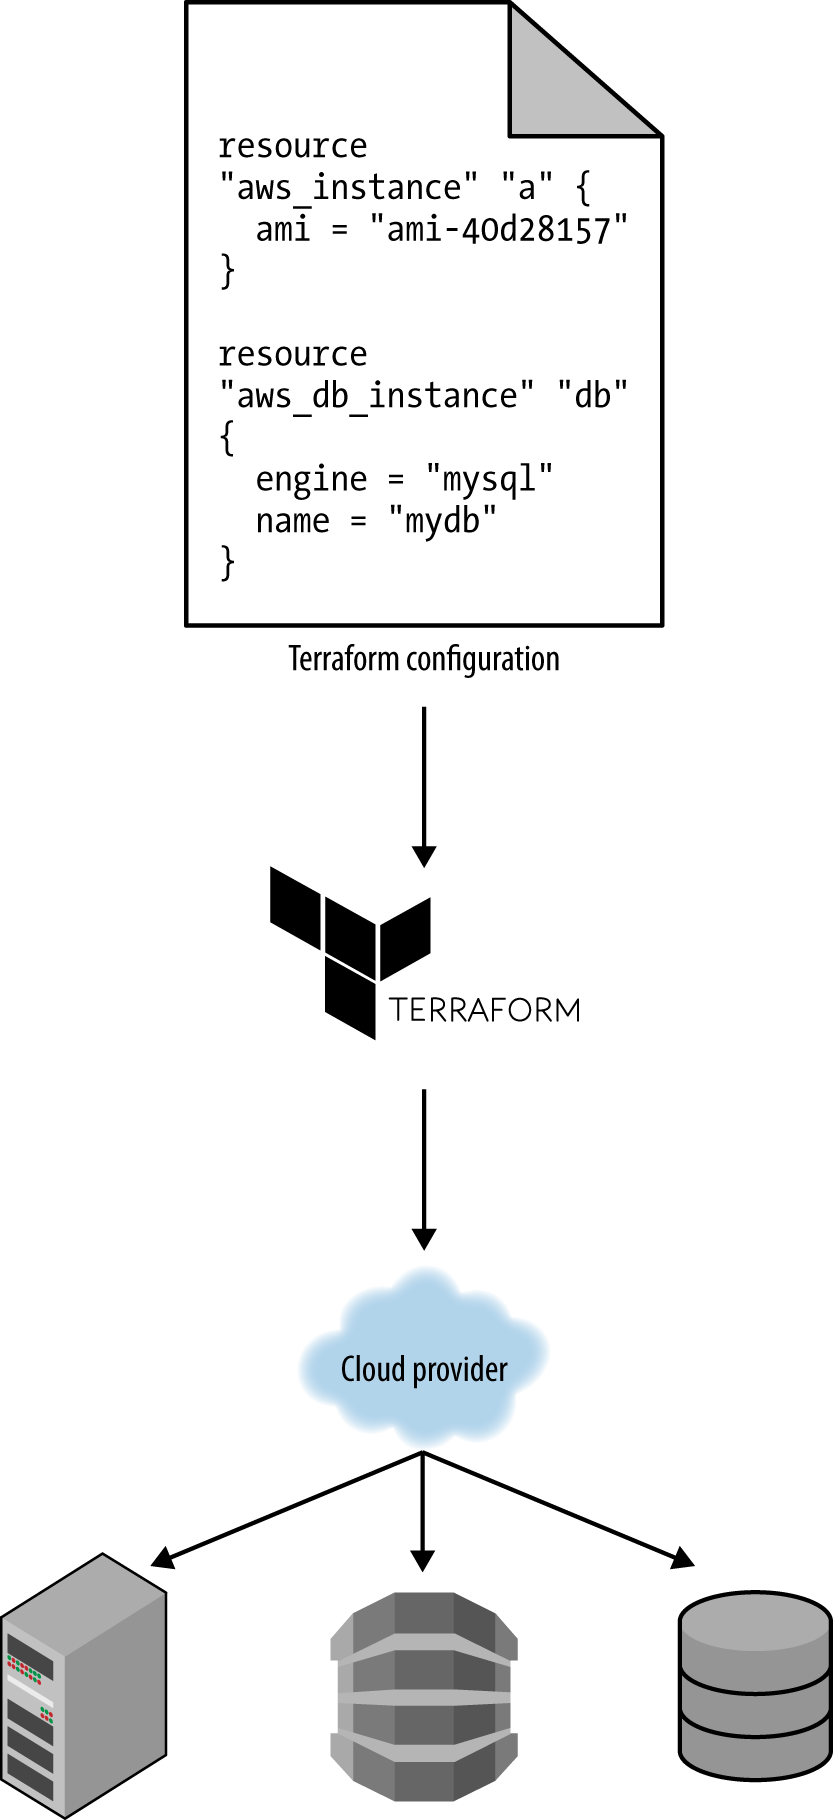
\includegraphics[width=0.5\textwidth]{figuras/terraform-working.png}
	 \vspace{-0.2cm}
	\\\textbf{\footnotesize Fonte: \cite{oreilly}}
	\label{fig:figura7}
\end{figure}
\vspace{-0.5cm}


\subsection{ Analise Comparativa }

Nesta seção é apresentada os itens de comparação. completar XXXXXXXXXXXXXXXX

\subsection{Fluxo de trabalho}
Os fluxos de trabalho  das ferramentas são bem simples e atendem equipes de diversos tamanhos. Este item descreve o fluxo principal de cada ferramenta. 

No fluxo de trabalho principal do \textbf{\textit{Terraform}}(veja na Figura \ref{fig:figura7}) possuem três etapas:

\begin{itemize}
  \item Definir: A definição de recursos da infraestrutura deve ser criada em qualquer editor de texto puro e salvo com a extensão \textbf{*.tf} respeitando a sintaxe do \textit{HCL}. É prática comum armazenar os arquivos em um repositório controlado por versão.
   \item Planejar: Visualizar as alterações antes de criar os recursos(aplicar).
   \item Aplicar/Destruir: Criar, atualizar ou deletar recursos na infraestrutura 
\end{itemize}


Este fluxo é resumido em três comandos  em três comandos \textbf{\textit{terraform init, terraform apply/destroy}}


\begin{itemize}

\item \textbf{\textit{terraform init }}: Este comando é usado somente na primeira vez quando é instalado ou quando o próprio \textit{terraform} solicita. Ele realiza \textit{download} de itens de funcionamento do \textit{terraform} como os \textit{providers, resource e modules} (\ref{terraform}). 

\item \textbf{\textit{terraform apply ou destroy }}: O terraform é detecta automaticamente as alterações de recursos, como, criação, atualização e exclusão e mostrar um plano do que ele fará antes de aplicar ou destruir recursos.

\end{itemize}

\begin{figure}[ht]
	\centering	
	\caption[\hspace{0.1cm}Fluxo Principal Terraform]{Fluxo Principal Terraform}
	\vspace{-0.4cm}
	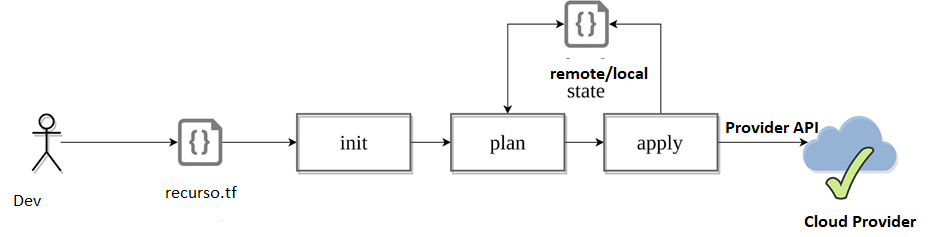
\includegraphics[width=1.2\textwidth]{artigo/figuras/terraform_single_workflow.png}
	 \vspace{-0.2cm}
	\\\textbf{\footnotesize Adaptado de: \cite{Turbinskii}}
	\label{fig:figura7}
\end{figure}
\vspace{-0.5cm}

Considerando apenas a função de provisionamento que o \textbf{\textit{Ansible}} tem. O fluxo de trabalho também é divido em duas etapas:

\begin{itemize}
  \item Desenvolvimento: Definir os recursos da infraestrutura que devem ser criados, este devem ser ser criados em qualquer editor de texto puro e salvos com a extensão \textbf{*.yaml}, respeitando a sintaxe dos \textit{Playbooks}. É prática comum armazenar os arquivos em um repositório controlado por versão.
  \item Aplicar/Destruir: Criar, atualizar ou deletar recursos na infraestrutura. 
\end{itemize}


Este fluxo é resumido em apenas um comando: \textbf{\textit{ansible-playbook recurso.yaml}}


A diferença entre o fluxo das duas ferramenta é que no \textit{Terraform} ele gera um arquivo de estado, com extensão \textbf{*.tfstate} que deve ser armazenado no controle de versão. Outra diferença é que no \textit{Ansible} o fluxo de destruir um recursos requer um \textit{Playbook} especifico para finalidade. Esta última diferença será explicada no item \ref{idem}.  


\subsection{Linguagem}

No \textit{Terraform}, um recurso é criado usando a linguagem personalizadas a \textit{HCL} e o mecanismo do \textit{Terraform} se encarrega de provisionar e atualizar recursos. Com o \textit{Ansible}, você usa a \textit{YAML} para expressar o estado desejado e o \textit{Ansible} se encarrega de criar o recurso oferece a você diferenças e uma maneira de atualizar robusta sua infraestrutura. Neste ponto o \textit{Ansible} tem uma certa vantagem, pois \textit{YAML} é muito usado por outras ferramentas.  No entando o \textit{Ansible} trabalha com o modelo de escrita de código procedural conforme mencionado no item \ref{procedural} o força ao usuário ter conhecimento prévio de como configurar uma determinado recurso antes de escrever um \textit{playbook}. 

\begin{comment}
\subsection{Documentação}

A documentação do \textit{Ansible} é bastante extensa e as vezes confusa e os exemplos não são completos e não acompanham as evoluções do produto, por outro lado existe uma grande quantidade de conteúdo disponível na internet, como blogs, vídeos, livros e cursos.

A documentação do \textit{Terraform} é bastante extensa completa os exemplos são claros e simples existe também muito conteúdo na internet.

\subsection{Performance}
\end{comment}
\subsection{Controle de Estado e Idempotência} \label{idem}
Um dos grandes de desafios das ferramentas de provisionamento é garantir que um determinado recursos seja único e que toda operação tenha o mesmo resultado esperado o que é chamando de idempotência tanto o  \textit{Terraform} quanto o \textit{Ansible} possuem essa característica. No \textit{Terraform} isto é implícito, pois o nome associado ao recursos tem que ser único, então o \textit{Terraform} faz o controle automaticamente pelo nome do recursos. No \textit{Ansible} essa característica é explicita deve-se ser informada na definição do recurso que ele deve ser único.

Uma característica observada no \textit{Terraform} é que ele mantém o estado da infraestrutura e detecta automaticamente alterações de estado e sincronizada a diferença entre o estado do \textit{Terraform} e a infraestrutura. Essa é uma grande vantagem em relação ao \textit{Ansible} que apresenta um modelo de recursos controlado, em que o usuário deve descreve o estado desejado ou seja, o usuário deve descrever que o recurso por exemplo deve ser excluído e o \textit{Ansible} entende como transformá-lo no estado desejado, diferente do \textit{Terraform} que apenas retirando o recurso do arquivo ele já entende que deve-se destruir o recurso na infraestrutura.

\subsection{Extensibilidade}

\textit{Ansible} e \textit{Terraform} possui um sistema de plugins e módulos permitem estender as suas funcionalidades. Este módulos e \textit{plugins} são escritos em linguagens de programação e pode ser compartilhados. As duas ferramentas possuem um repositório central, no \textit{Ansible} é chamado de \textit{Galaxy} e no \textit{Terraform} é chamado como \textit{Registry} onde esses módulos e \textit{plugins} pode ser compartilhados para que outras pessoas possam usar. No \textit{Terraform} o usuário só pode escrever um módulo em apenas uma linguagem de programação a \textit{Golang}  \footnote{Linguagem de programação de propósito geral desenvolvida pela Google} e no \textit{Ansible} é permitido usar qualquer linguagem de programação.  

A vantagem de se poder usar qualquer linguagem para a extensibilidade permite-se usar uma linguagem em que uma organização já utiliza o que diminui a curva de aprendizado e não ter a necessidade de aprender novas linguagens de programação.  

\subsection{Performance}
A medida em que sistemas se desenvolvem as quantidades de recursos requeridos podem aumentar ou diminuir. A velocidade em que esses recursos são criados, destruídos ou atualizados, podem por exemplo, podem ocasionar em instabilidades, quedas de serviços, comprometendo o \textit{LNS} \footnote{ \textit{LNS}: Acordo de Nível de Serviço} de um sistema. É importante garantir que mudanças na infraestrutura sejam simples e rápidas. Um software de provisionamento deve ser eficaz a ponto de não compromenter toda uma atualização de recurso. Neste trabalho a medição da performance foi dada pelo tempo em minutos em que um recurso(utilizou-se apenas máquinas virtuais que é um recurso mais criado) é criado no fornecedor de computação na nuvem. As tabelas \ref{tab:tabela1} e \ref{tab:tabela2} a seguir mostram uma comparação entre \textit{Ansible} e \textit{terraform}. 


% Tabela
\begin{table}[ht]
	\centering
	\caption{\hspace{0.1cm} Comparativo - Criação de Recurso}
	\vspace{-0.3cm} % espaço entre titulo e tabela
	\label{tab:tabela1}
	% Conteúdo da tabela
	\begin{tabular}{l|c|c}
  \hline
    \textbf{Qtde. Recursos}	& \textbf{Tempo - Ansible} & \textbf{Tempo - Terraform} \\
    \hline
  1   & 1.5  Minutos   & 0.4  Minutos    \\
2   & 2.10  Minutos   & 1.5  Minutos    \\
3   & 3.17  Minutos   & 2.1  Minutos    \\
5   & 5.32  Minutos   & 4.7  Minutos     \\
10  & 10.3 Minutos   & 5.2  Minutos      \\
15  & 13.8  Minutos   & 5.7 Minutos      \\
20  & 16.6  Minutos   & 7.38  Minutos      \\

     \hline
 \end{tabular}
 	\vspace{.1cm}  %espaço entre tabela e fonte
	\small
	% Fonte
	{\footnotesize\\ \textbf{Fonte: Próprio Autor}}
\end{table}


% Tabela
\begin{table}[ht]
	\centering
	\caption{\hspace{0.1cm} Comparativo - Destruição de Recurso}
	\vspace{-0.3cm} % espaço entre titulo e tabela
	\label{tab:tabela2}
	% Conteúdo da tabela
	\begin{tabular}{l|c|c}
  \hline
    \textbf{Qtde. Recursos}	& \textbf{Tempo - Ansible} & \textbf{Tempo - Terraform} \\
    \hline
  1   & 1.2  Minutos   & 0.4  Minutos    \\
2   & 1.9    Minutos   & 1.2  Minutos    \\
3   & 2.5    Minutos   & 1.6  Minutos    \\
5   & 3.6    Minutos   & 2.7  Minutos     \\
10  & 4.20   Minutos   & 3.2  Minutos      \\
15  & 5.8    Minutos   & 4.19 Minutos      \\
20  & 7.4    Minutos   & 5.1  Minutos      \\

     \hline
 \end{tabular}
 	\vspace{.1cm}  %espaço entre tabela e fonte
	\small
	% Fonte
	{\footnotesize\\ \textbf{Fonte: Próprio Autor}}
\end{table}


A titulo de comparação, para se criar uma máquina virtual no console do fornecedor leva-se um tempo estimado de 1 minutos, entre escolher os requisitos da máquina, como sistema operacional, quantidade de memória RAM, tamanho e tipos de disco rígidos. 

Nesta comparação o \textit{Terraform} tem uma melhor performance, tanto para criação ou destruição de recursos. Um fato para essa diferença de performance é fato dele distribuir as execuções(criação ou destruição de recursos) por núcleo. 

Segundo a \cite{hashcorp03} "Nossa regra prática é 10 execuções \textit{Terraform} por núcleo de CPU, com 2 núcleos de CPU alocados para os serviços básicos.  Portanto, uma máquina de 8 núcleos com 8 GB de memória pode executar confortavelmente 20 execuções \textit{Terraform}."

A comparação ficou limitada em 20 máquinas virtuais, devido ao valores em dólares disponíveis para a realização dos testes. 

\subsection{Outra Comparações}
\textit{Ansible} e \textit{Terraform} são ferramentas de código aberto e código fonte de ambas estão no hospedadas no \textit{Github}. O \textit{github} é um repositório central de código fonte, onde existem atualmente mais de 40 milhões de usuários e mais de 10 milhões de projetos e pessoas do mundo inteiro podem contribuir com projetos de código aberto. No \textit{Github} é possível extrair métricas de projetos como: 

\begin{itemize}
    \item  \textit{Contributors}: Número de pessoas que contribuíram de alguma forma no projeto, corrigindo \textit{bugs}, adicionando novas funcionalidades.
     \item \textit{Issues}: Número de problemas encontrados por outras pessoas e relatados ao projeto. 
     \item \textit{Code Frequency}: Número de linhas de código inseridas no código fonte principal anualmente. 
\end{itemize}

A tabela a seguir foi montada com base nas métricas fornecidas do \textit{Github}: 
   
  
\begin{table}[ht]
	\centering
	\caption{\hspace{0.1cm} Github - Insights}
	\vspace{-0.3cm} % espaço entre titulo e tabela
	\label{tab:tabela2}
	% Conteúdo da tabela
	\begin{tabular}{l|c|c}
  \hline
    \textbf{Métrica}	& \textbf{Ansible} & \textbf{Terraform} \\
    \hline
  Contributors & 4.752  & 1351\\
  Issues   & 4.200   & 1103     \\
  Code Frequency  & 200MIL  &   100MIL  \\
     \hline
 \end{tabular}
 	\vspace{.1cm}  %espaço entre tabela e fonte
	\small
	% Fonte
	{\footnotesize\\ \textbf{Fonte: Próprio Autor}}
\end{table}




\subsection{Conclusão e Trabalho Futuros}
A detecção de estado automático é um grande diferencial do terraform, pois o gerenciamento de código se torna simples, uma vez que não é necessário conhecido os passo necessários para se chegar no estado final desejado.

